\section{Introduction}
Perverse schobers are a categorification of perverse sheaves, initially proposed by Kapranov-Schechtman \cite{kapranovPerverseSchobers2015}. Just as perverse sheaves organize vector space invariants such as those arising in symplectic geometry and representation theory, perverse schobers are expected to organize categorical invariants. Much work has since gone into realizing this proposal in various settings \cites{bondalPerverseSchobersBirational2018,christGinzburgAlgebrasTriangulated2022,kapranovPerverseSchobers2015,dyckerhoffPerverseSchobersCoxeter2025}, although a general definition is still not available.

These categorifications, while ad hoc, follow a common recipe. First, one finds a description of the corresponding category of perverse \textit{sheaves} in terms of diagrams of abelian groups with relations. Then, one can consider diagrams of stable $\one$-categories of the same shape, and categorify relations following certain rules of categorification, established through these examples. Such rules can be found tabulated in \cite{christLaxAdditivity2025}*{\S 1.1}.

Studying the first step more carefully, one observes that these diagrammatic descriptions of perverse sheaf categories are very often of a microlocal origin. That is, the abelian groups are microstalks, and the arrows are communications of microstalks. Gelfand--MacPherson--Vilonen \cite{gelfandMicrolocalPerverseSheaves2005} take advantage of this perspective and present a possible approach to describe any perverse sheaf category as a diagram category, with no reference to derived categories or $t$-structures.

Therefore it is natural to expect that a general and uniform definition of perverse schobers can be achieved by categorifying this approach. The aim of this paper is to begin to develop a microlocal theory of perverse schobers, motivated by this expectation.

\subsection{Microlocal sheaves}
Microlocal sheaf theory \cite{kashiwaraSheavesManifolds1990} is an enhancement of sheaf theory which views sheaves on a smooth real manifold $X$ as living over the symplectic manifold $T^*X$. More precisely, the theory upgrades the support of a sheaf $\calF$ to a microsupport, which is a closed, conic subset inside $T^*X$. Thus given a closed, conic subset $\Lambda$, one can define a subcategory of the stable $\infty$-category $\sh(X)$ of sheaves valued in $\bbZ$,
\[\sh_{\Lambda}(X)\subseteq \sh(X),\]
consisting of those sheaves whose microsupport is contained in $\Lambda$. For example, given a reasonable stratification $\calS$ of $X$, $\sh_{T^*_\calS X}(X)$ is the subcategory of sheaves constructible with respect to $\calS$.

We can localize $\sh_{\Lambda}(X)$ into a presheaf of categories over $T^*X$, denoted
\[\Omega\mapsto \sh_{\Lambda}(X;\Omega) := \sh_{\Omega^c\cup \Lambda}(X)/\sh_{\Omega^c}(X).\]
By sheafification, we obtain a sheaf of categories that we denote $\mush_{\Lambda}(-)$, whose sections we refer to as microlocal sheaves. There is a precise sense in which microlocal sheaves are independent of the particular polarization. This is exhibited by quantized contact transformations as explained in \cite{kashiwaraSheavesManifolds1990}*{Chapter VII}.

For points $p\in \Lambda$ that are in generic position, microlocal cut-offs let us present the stalk $\mush_{\Lambda}(p)$ as a quotient category,
\begin{equation}\label{equation:cutoff}
    \mush_{\Lambda}(p)\simeq \sh_{0_U\cup \Lambda}(U)/\Loc(U),
\end{equation}
where $U$ is a small open neighbourhood of the projection $\pi(p)\in X$, and $0_U$ is the zero section.

\subsection{Microlocal perverse sheaves}\label{subsection:muperv}
If $X$ is a smooth complex manifold and $\Omega$ is $\bbC^\times$-conic then there is a subcategory of microlocal perverse sheaves
\[\muPerv_{\Lambda}(\Omega)\subset \mush_{\Lambda}(\Omega),\]
which organize into a sheaf of categories $\muPerv_{\Lambda}(-)$, as studied in \cites{andronikofMicrolocalVersionRiemannHilbert1994,gelfandMicrolocalPerverseSheaves2005,waschkiesMicrolocalPerverseSheaves2002,waschkiesStackMicrolocalPerverse2004,cotePerverseMicrosheaves2025}.

Microlocal perverse sheaves are particularly tractable near a point $p\in\Lambda$ in generic position -- that is, where
\[\pi^{-1}(\pi(p))\cap \Lambda = \bbC^\times p.\]
Near such $p$, the entire geometry is visible on the base; there is a hypersurface germ $H$ defined on a neighbourhood $U$ of $\pi(p)$, such that $\Lambda=\Lambda_H$ near $\bbC^\times p$, where $\Lambda_H$ denotes the closure of the conormal of the smooth locus of $H$. Waschkies \cite{waschkiesStackMicrolocalPerverse2004} uses microlocal cut-offs to prove an analog of (\ref{equation:cutoff}),
\[\muPerv_{\Lambda}(\bbC^{\times}p)\simeq \Perv_{\Lambda_H}(U)/\Loc(U).\]
We may choose local coordinates $x_1,\dots,x_{N-1},y$ on $U$ such that $\pi(p) = (0,\dots,0)$ and such that $H$ is cut out by an equation of the form
\begin{equation}\label{equation:equation}
    y^m + \text{ higher order terms}.
\end{equation}

Gelfand--MacPherson--Vilonen \cite{gelfandMicrolocalPerverseSheaves2005} show that $\Perv_{\Lambda_H}(U)/\Loc(U)$ has an intrinsically abelian description. Geometrically, the pair $(U,H)$ can be viewed as a family of discs $(\bbC,R)$ parameterized by $(x_1,\dots,x_{N-1})$, where $R\subset \bbC$ is a finite set of points, see Figure~\ref{figure:y2x4}. They explain that $\Perv_{\Lambda_H}(U)/\Loc(U)$ can be constructed out of the categories $\Perv(\bbC,R)/\Loc(\bbC)$. In turn, a quiver description of $\Perv(\bbC,R)/\Loc(\bbC)$ is given in \cite{gelfandPerverseSheavesQuivers1996}, which is intrinsically abelian. Let us refer to this description as the local GMV construction.

\begin{rmk}[Microlocal perverse sheaves at non-generic points]\label{rmk:gmvfull}
    By applying a suitable contact transformation, any point $p\in\Lambda$ can be made generic and thus understood via a pair $(U,H)$ as above. Moreover, if $p\in\Lambda$ is a codimension $\leq i$ singularity, then we can reduce the dimension so that $U$ has dimension $i+1$. The main result of \cite{gelfandMicrolocalPerverseSheaves2005} uses this to give an intrinsically abelian construction of the sheaf of categories $\muPerv_{\Lambda}(-)$ on the open locus $\Lambda^{\leq 1}\subseteq \Lambda$ of singularities of codimension $\leq1$ in terms of pairs of the form $(U\subset \bbC^2,C)$.
\end{rmk}

\begin{figure}
    \caption{Pair $(\bbC^2_{x,y},C)$ together with discs $(\bbC_y,R)$ parametrized by $x$}
    \label{figure:y2x4}
    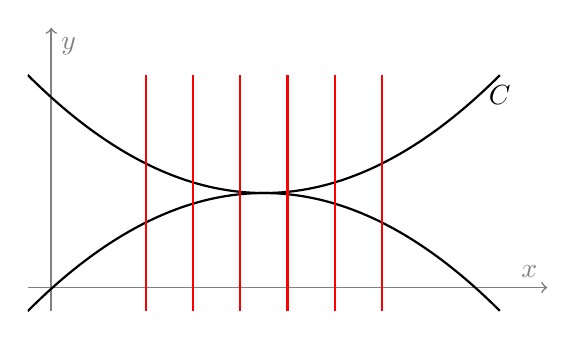
\begin{tikzpicture}[scale=3]
    % Define bounding clip area (-1 < x < 1, -0.5 < y < 1)
    \clip (-1, -0.5) rectangle (1.2, 0.7);

    % Draw unlabelled coordinate axes at x = -0.9 and y = -0.4
    \draw[->, gray, line width=0.6pt] (-1, -0.4) -- (1.2, -0.4) node[above left, gray] {$x$};% Horizontal axis
    \draw[->, gray, line width=0.6pt] (-0.9, -0.5) -- (-0.9, 0.7) node[below right, gray] {$y$};% Vertical axis

    % Graph of y = 0 (black line along the x-axis)
    %\draw[black, thick] (-1, 0) -- (1, 0);

    % Graph of y = x^2 in black
    \draw[black, thick, domain=-1:1, samples=100] plot (\x, {0.5*\x*\x}) node[below, black] {$C$};
    \draw[black, thick, domain=-1:1, samples=100] plot (\x, {-0.5*\x*\x});
    %\draw[black, thick, domain=-1:1, samples=100] plot (\x*\x, {0.5*\x*\x*\x}) node[below, black] {$C$};

    % Vertical red line at x = 0.5
    \draw[red, thick] (-0.5, -0.5) -- (-0.5, 0.5);
    \draw[red, thick] (-0.3, -0.5) -- (-0.3, 0.5);
    \draw[red, thick] (-0.1, -0.5) -- (-0.1, 0.5);
    \draw[red, thick] (0.1, -0.5) -- (0.1, 0.5);
    \draw[red, thick] (0.3, -0.5) -- (0.3, 0.5);
    \draw[red, thick] (0.5, -0.5) -- (0.5, 0.5);
    \end{tikzpicture}
\end{figure}

\subsection{The aim of this paper}
The main objective of this paper is to categorify the quotient category $\Perv_{\Lambda_H}(U)/\Loc(U)$ to a $\two$-category of microlocal perverse schobers, which we denote
\[\olsftwoP_{\Lambda_H}(U),\]
where as before, $H$ is a hypersurface germ defined on a small open subset $0\in U\subset \bbC^N_{x_1\dots,x_{N-1},y}$ by an equation of the form (\ref{equation:equation}).

From the discussion in \S\ref{subsection:muperv}, this should be thought of as giving a definition of microlocal perverse schobers defined near $\bbC^\times p$ for any $p\in\Lambda$ generic. For the rest of the introduction, we will assume that the base has dimension 2 so that $U=U_{x,y}$ and $H=C$ is a curve. We broadly partition our objective into three steps.

\begin{itemize}
    \item Step 1: Categorify $\Perv(\bbC,R)/\Loc(\bbC)$ to $\olsftwoP(\bbC,R)$, together with a projection functor $\sftwoP(\bbC,R)\to \olsftwoP(\bbC,R)$.
    \item Step 2: Categorify $\Perv_{\Lambda_C}(U)/\Loc(U)$ to $\olsftwoP_{\Lambda_C}(U)$.
    \item Step 3: Exhibit invariance under contact transformations.
\end{itemize}

Steps 1 and 2 constitute the construction of $\olsftwoP_{\Lambda_C}(U)$ via a categorification of the local GMV construction.

Step 3 is where our categorification is scrutinized. Recall that microlocal perverse sheaves are defined ``top down'' with contact invariance also inherited in this way, while the ``bottom up'' approach of GMV can be thought of as an alternative construction. In contrast, we take the ``bottom up'' approach as the \textit{definition} of microlocal perverse schobers, and to argue that this definition is a good one, we should exhibit contact invariance directly.

In this paper, we study a particularly interesting contact transform. We recall that there is a canonical contact transform
\[T^*\bbP^2 - 0_{\bbP^2}\simeq T^*\check{\bbP}^2 - 0_{\check{\bbP}^2},\]
where $\check{\bbP}^2$ is the dual projective space, parametrizing lines in $\bbP^2$. Moreover, if $C\subset \bbP^2$ is a projective curve, then we may consider its projective dual curve $\check{C}\subset\check{\bbP}^2$, parametrizing (limits of) tangent lines to $C$. Under the contact transform, $\Lambda_{C}$ identifies with $\Lambda_{\check{C}}$. In the perverse sheaf setting, this quantizes to the Radon transform \cite{kiehlLefschetzTheoryBrylinskiRadon2001},
\[\Perv_{0_{\bbP^2}\cup \Lambda_{C}}(\bbP^2)/\Loc(\bbP^2)\simeq \Perv_{0_{\check{\bbP}^2}\cup \Lambda_{\check{C}}}(\check{\bbP}^2)/\Loc(\check{\bbP}^2).\]

More locally, we may associate to our pair $(U_{x,y},C)$, a dual pair $(V_{a,b},\check{C})$, where $\check{C}\subset V_{a,b}$ is the germ of the curve near $(0,0)$ which parametrizes (limits of) tangent lines $y=ax-b$ to $C$. Figure~\ref{figure:radon} illustrates a pair of dual curves. We record below the resulting special case of Step 3.
\begin{itemize}
    \item Step 3': Construct a Radon transform equivalence, $\olsftwoP_{\Lambda_C}(U)\simeq \olsftwoP_{\Lambda_{\check{C}}}(V)$.
\end{itemize}
We note that the Radon transform is in some sense typical, and highlights difficulties that we may encounter for general contact transformations. In a related context, the Radon transform plays a key role in \cites{beilinson2016constructible,saitoSingularSupportsMixed2025} to develop a theory of singular support for \'etale constructible sheaves.

\begin{figure}[ht]
    \caption{A curve $C$ and its dual $\check{C}$}
    \label{figure:radon}

    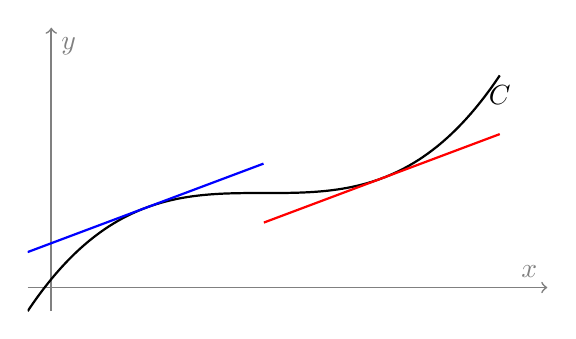
\begin{tikzpicture}[scale=3]
    % Define bounding clip area (-1 < x < 1, -0.5 < y < 1)
    \clip (-1, -0.5) rectangle (1.2, 0.7);

    % Draw unlabelled coordinate axes at x = -0.9 and y = -0.4
    \draw[->, gray, line width=0.6pt] (-1, -0.4) -- (1.2, -0.4) node[above left, gray] {$x$};% Horizontal axis
    \draw[->, gray, line width=0.6pt] (-0.9, -0.5) -- (-0.9, 0.7) node[below right, gray] {$y$};% Vertical axis

    % Graph of y = 0 (black line along the x-axis)
    %\draw[black, thick] (-1, 0) -- (1, 0);

    % Graph of y = x^2 in black
    %\draw[black, thick, domain=-1:1, samples=100] plot (\x, {0.5*\x*\x}) node[below, black] {$C$};
    %\draw[black, thick, domain=-1:1, samples=100] plot (\x, {-0.5*\x*\x});
    \draw[black, thick, domain=-1:1, samples=100] plot (\x, {0.5*\x*\x*\x}) node[below, black] {$C$};

    \draw[red, thick, domain=0:1, samples=100] plot (\x, {1.5*0.5*0.5*\x-0.5*0.5*0.5});
    \draw[blue, thick, domain=-1:0, samples=100] plot (\x, {1.5*0.5*0.5*\x+0.5*0.5*0.5});
    % Vertical red line at x = 0.5
    % \draw[red, thick] (0.5, -0.5) -- (0.5, 0.5) node[below left, red] {$a=a_0$};
    \end{tikzpicture}
    \begin{tikzpicture}[scale=3]
    % Define bounding clip area (-1 < x < 1, -0.5 < y < 1)
    \clip (-1, -0.5) rectangle (1.2, 0.7);

    % Draw unlabelled coordinate axes at x = -0.9 and y = -0.4
    \draw[->, gray, line width=0.6pt] (-1, -0.4) -- (1.2, -0.4) node[above left, gray] {$a$};% Horizontal axis
    \draw[->, gray, line width=0.6pt] (-0.9, -0.5) -- (-0.9, 0.7) node[below right, gray] {$b$};% Vertical axis

    % Graph of y = 0 (black line along the x-axis)
    %\draw[black, thick] (-1, 0) -- (1, 0);

    % Graph of y = x^2 in black
    %\draw[black, thick, domain=-1:1, samples=100] plot (\x, {0.5*\x*\x}) node[below, black] {$C$};
    %\draw[black, thick, domain=-1:1, samples=100] plot (\x, {-0.5*\x*\x});
    \draw[black, thick, domain=-1:1, samples=100] plot (\x*\x, {0.5*\x*\x*\x}) node[below, black] {$\check{C}$};

    % Vertical red line at x = 0.5
    %\draw[red, thick] (0.5, -0.5) -- (0.5, 0.5);
    \fill[red] (0.5,0.5*0.5*0.707) circle (0.5pt);
    \fill[blue] (0.5,-0.5*0.5*0.707) circle (0.5pt);
    \end{tikzpicture}
\end{figure}

\subsection{Radon transform and symplectic suspension}
We illustrate the main new phenomenon which arises when we attempt this categorification procedure in a key example. We begin by considering two possible categorifications of $\Perv(\bbC,0)/\Loc(\bbC)$ at Step 1. We note that both of these are equipped with projection functors from $\sftwoP(\bbC,0)$.
\begin{enumerate}
    \item The first is the quotient $\two$-category $\olsftwoP^{\opname{monad}}(\bbC,0) := \sftwoP(\bbC,0)/\sftwoL(\bbC)$. It turns out that this is abstractly equivalent to the $\two$-category whose objects are pairs $(\Phi,M)$ where $\Phi$ is a stable $\one$-category, and $M$ is a monad on $\Phi$ such that $\coCone(\id\to M)$ is an autoequivalence.
    \item Recall that $\Perv(\bbC,0)/\Loc(\bbC)$ is abstractly equivalent to the category of pairs $(W,t)$ where $W$ is a $k$-vector space and $t$ is an automorphism of $W$. Our second categorification $\olsftwoP^{\opname{aut}}(\bbC,0)$ is the $\two$-category of pairs $(\Phi,T)$ where $\Phi$ is a stable $\one$-category and $T$ is an autoequivalence of $\Phi$.
\end{enumerate}

Let $C=\{y=x^2\}$. For this curve, Step 2 is easy. Given our categorification $\olsftwoP(\bbC,0)$ from Step 1, the categorified local GMV construction simply defines
\[\olsftwoP_{\Lambda_C}(U) := \olsftwoP(\bbC,0),\]
because $C$ is smooth. The dual curve $\check{C} = \{b=a^2/4\}$ is also smooth so,
\[\olsftwoP_{\Lambda_{\check{C}}}(V) := \olsftwoP(\bbC,0).\]
Thus the Radon transform of Step 3' is identified with an equivalence of $\two$-categories, which we denote
\[\calRadon:\olsftwoP(\bbC,0)\simeq \olsftwoP(\bbC,0).\]
We emphasize that the Radon transform happens on the 2-dimensional geometry of $(U,C)$ and not the 1-dimensional geometry of $(\bbC,0)$.

While these two $\two$-categories are obviously equivalent, we claim that the Radon transform ought to be a different operation which we call symplectic suspension. Assuming that $k=\bbC$, let us denote by $\ol{\calF}(M,f) \in \olsftwoP(\bbC,0)$ the image of the Lefschetz schober associated to a Lefschetz fibration $(M,f)$, under the projection functor constructed in Step 1. We posit that the Radon transform should agree with the symplectic suspension operation,
\[\calRadon:\ol{\calF}(M,f)\mapsto \ol{\calF}(M\times\bbC_z,f+z^2).\]
In \S\ref{subsection:suspension}, we define an algebraic version of the symplectic suspension (general to any $k$), as a functor $\calSus: \sftwoP(\bbC,0)\to \sftwoP(\bbC,0)$, which conjecturally satisfies
\[\calSus:\calF(M,f)\mapsto \calF(M\times\bbC_z,f+z^2).\]
So more precisely, we posit that the Radon transform is compatible with $\calSus$ via projection functors as illustrated in the following commutative diagram.

% https://q.uiver.app/#q=WzAsNCxbMCwwLCJcXHNmdHdvUChcXGJiQywwKSJdLFsxLDAsIlxcc2Z0d29QKFxcYmJDLDApIl0sWzAsMSwiXFxvbHNmdHdvUChcXGJiQywwKSJdLFsxLDEsIlxcb2xzZnR3b1AoXFxiYkMsMCkiXSxbMCwyXSxbMSwzXSxbMCwxLCJcXGNhbFN1cyJdLFsyLDMsIlxcb3BuYW1le1JhZG9ufSJdXQ==
\[\begin{tikzcd}[ampersand replacement=\&]
	{\sftwoP(\bbC,0)} \& {\sftwoP(\bbC,0)} \\
	{\olsftwoP(\bbC,0)} \& {\olsftwoP(\bbC,0)}
	\arrow["\calSus", from=1-1, to=1-2]
	\arrow[from=1-1, to=2-1]
	\arrow[from=1-2, to=2-2]
	\arrow["{\calRadon}", from=2-1, to=2-2]
\end{tikzcd}\]

If we choose the first categorification, then $\calRadon$ is determined to be the functor
\begin{align*}
    \calSus_{\opname{monad}}:\olsftwoP^{\opname{monad}}(\bbC,0)&\to \olsftwoP^{\opname{monad}}(\bbC,0)\\
    (\Phi,M)&\mapsto (\Phi,\id_\Phi\times_M\id_\Phi)
\end{align*}
However, this is not an equivalence as some data of the monad is lost. If instead we choose the second categorification, then $\calRadon$ is determined to be the functor
\begin{align*}
    \calSus_{\opname{aut}}:\olsftwoP^{\opname{aut}}(\bbC,0)&\to \olsftwoP^{\opname{aut}}(\bbC,0)\\
    (\Phi,T)&\mapsto (\Phi,T[-1])
\end{align*}
which is clearly an equivalence. So we learn that $\olsftwoP^{\opname{aut}}(\bbC,0)$ is the correct categorification at Step 1. We will prove in Theorem~\ref{thm:limit0} that in fact, we may recover the correct categorification from the incorrect one by inverting $\calSus_{\opname{monad}}$ as follows.

\begin{thm}\label{thm:introcolimit}
    There is a natural diagram of $\two$-categories,
    \[\olsftwoP^{\opname{aut}}(\bbC,0)\to \cdots\to \xto{\calSus_{\opname{monad}}}\olsftwoP^{\opname{monad}}(\bbC,0)\xto{\calSus_{\opname{monad}}}\olsftwoP^{\opname{monad}}(\bbC,0)\]
    which exhibits $\olsftwoP^{\opname{aut}}(\bbC,0)$ as a limit.
\end{thm}

Concretely, this says that the part of the monad $M$ stable under $\calSus_{\opname{monad}}$ is precisely the autoequivalence $T:=\coCone(\id\to M)$. We summarize as follows.

\begin{moral}\label{moral:intromain}
    The correct categorification of the quotient ${\Perv}(\bbC,0)/Loc(\bbC)$ is not the quotient of the categorifications, but we can correct this by inverting the symplectic suspension in the manner above.
\end{moral}

This is reflected in our choice to denote the categorification by $\olsftwoP(\bbC,0)$ instead of $\ol{\sftwoP}(\bbC,0)$.

\subsection{Radon transform for \texorpdfstring{$y^m=x^n$}{y\^{}m=x\^{}n}}
The main example of Radon transform that we study in this paper is for the curve $C=\{y^m = x^n\}$ where $0<m<n$. The dual curve is given by
\[\check{C} = \{\left(\frac{m}{n-m}b\right)^{n-m} = \left(\frac{m}{n}a\right)^n\}.\]
Ignoring constants, this is $\{b^{n-m} = a^n\}$, a curve of the same form with $m$ replaced by $n-m$. This curve has been studied in various related contexts, for example, \cites{oblomkovHilbertSchemePlane2012,macphersonPerverseSheavesSingularities1988}.

Let us view $(\bbC^2_{x,y},C)$ as a family of discs. Over $x=1$, we see the disc $(\bbC_y,\{y^m=1\})$. As $x$ makes one revolution around the unit circle, the points cyclically rotate through an angle of $2\pi n/m$, forming the $(n,m)$-torus link. This geometry is reflected in the following description of $\olsftwoP(\bbC^2_{x,y},C)$; its objects are given by
\begin{enumerate}
    \item a stable $\infty$-category $\Phi$,
    \item an $n$-periodic $m$-term $\infty$-admissible SOD $\Phi = \langle\Phi_1,\dots,\Phi_m\rangle$, and
    \item\label{item:ignore} an autoequivalence $T:\Phi\to \Phi$ which is ``conjugate-compatible with respect to this SOD''.
\end{enumerate}
We will ignore (\ref{item:ignore}) for the rest of this discussion. Consider the mutations,
\[\langle\Phi_1,\dots,\Phi_m\rangle = \langle\Phi_2,\dots,\Phi_{m+1}\rangle = \langle\Phi_3,\dots,\Phi_{m+2}\rangle\cdots.\]
The SOD is said to be $n$-periodic if $\Phi_{i} = \Phi_{i+n}$ for all $i\geq1$. When $m=2$, this specializes to the notion introduced by Dyckerhoff--Kapranov--Schechtman \cite{dyckerhoffNsphericalFunctorsCategorification2023}.

Repeating this analysis for the dual curve $\check{C}$ and continuing to ignore autoequivalences, we formulate the following variant of the Radon transform for $C$. The proof can be extracted from that of the original Radon transform for $C$, which appears in the main text as Theorem~\ref{thm:ykxnschober}.
\begin{thm}\label{thm:radonsod}
    Let $\sfSOD(m)^{n\mathrm{-periodic}}$ denote the collection of pairs $(\Phi,\frakS)$ consisting of a stable $\one$-category $\Phi$ and an $m$-term SOD $\frakS$ which is $\infty$-admissible and $n$-periodic. Then, there is a natural bijection,
    \[\sfSOD(m)^{n\mathrm{-periodic}}\simeq \sfSOD(n-m)^{n\mathrm{-periodic}}.\]
\end{thm}

\begin{eg}\label{eg:introx3y2}
    Let $n=3$ and $m=2$. By \cite{dyckerhoffNsphericalFunctorsCategorification2023}, $3$-periodic 2-term SODs are those for which the gluing functor is an equivalence, thus are described by a single category. On the other hand, a 3-periodic 1-term SOD is also just a single category.
\end{eg}

It is proposed in \cite{dyckerhoffNsphericalFunctorsCategorification2023} that forming iterated mutations of a 2-term SOD is a categorical counterpart of the procedure of forming continued fractions, which in turn are related to iterated products of matrices of the form
\[\begin{bmatrix}
0 & -a_0\\
1 & -a_1
\end{bmatrix}.\]
Extending this slogan, Kapranov (in personal communication) proposed that forming iterated \textit{cyclic} mutations of an $m$-term SOD is a categorical counterpart of forming $m$-ary generalized continued fractions as studied by Jacobi \cites{bernstein2006jacobi,lehmerJacobisExtensionContinued1918}, which in turn are related to iterated products of $m\times m$ companion matrices,
\[\begin{bmatrix}
0 & \cdots & 0 & -a_0\\
1 & \cdots & 0 & -a_1\\
\vdots & \ddots & \vdots & \vdots\\
0 & \cdots & 1 & -a_{m-1}
\end{bmatrix}.\]
With this in mind, we have the following decategorification of Theorem~\ref{thm:radonsod}.

\begin{prop}
    Let $k$ be a field. Let $P(m,n)$ denote the set of $n$-tuples $(A_1,\dots,A_n)$ of $m\times m$ companion matrices that satisfy $A_n\cdots A_2A_1 = I$. Then, there is a natural bijection,
    \[P(m,n)\simeq P(n-m,n).\]
\end{prop}

\begin{proof}
    We show that there is a bijection $P(m,n)\simeq \Pi(m,n)$ where $\Pi(m,n)\subset \opname{Gr}(m,n)$ is the open positroid locus. These are those objects for which when represented by an $n\times m$ matrix, any $m$ cyclically consecutive rows have a non-zero minor.
    
    Denote by $e_1\in k^m$ the first standard basis vector and define recursively $e_{i+1} = A_ie_i$ for $i\geq 1$. See that $e_1,\dots,e_m$ is the standard basis, that $e_{i+n}=e_i$ for all $i$, and that any $m$ consecutive vectors in this sequence form a basis. Thus the assignment
    \[(A_1,\dots,A_n)\mapsto [e_1|e_2|\cdots |e_n]^{\intercal}\]
    defines a map $P(m,n)\to \Pi(m,n)$, which is easily seen to be a bijection. We are done by recalling the natural bijection
    \[\Pi(m,n)\simeq \Pi(n-m,n)\]
    by taking the orthogonal subspace under the standard bilinear form on $k^n$.
\end{proof}

We note that $\Pi(m,n)$ also appears as a moduli of microlocal sheaves supported on a Legendrian torus link in $\bbR^2$ as explained in \cite{shendeClusterVarietiesLegendrian2019}. Work of Kuwagaki \cite{kuwagakiCategorificationLegendrianKnots2019} studies perverse schobers in the real microlocal setting, where $n$-periodic SODs naturally arise from the same Legendrian torus links. This picture is related to $(\bbC^2,C)$ via the Fourier transform of Kapranov--Soibelman--Soukhanov \cite{kapranovPerverseSchobersAlgebra2020}. In fact, this is the geometry which implicitly underlies the proof of Theorem~\ref{thm:radonsod}, presented in \S\ref{subsection:ykxn}. Ongoing work explores this relation further.

\subsection{Main constructions and results}
We first outline our main constructions. We recall from \cite{kapranovPerverseSchobers2015} that to define perverse schobers on $(\bbC,R)$, we make a choice of cuts and write down a certain diagram of categories, which we shall call an abstract perverse schober. An action of the braid group on the set of abstract schobers encodes how diagrams corresponding to different choices of cuts are related, leading to a definition independent of the choice of cuts.

Upgrading this, we will construct $\two$-categories together with functors and compatible braid group actions,
\[\sfSph(n)\to\sfSphMnd(n)\to\sfAut(n).\]
such that a $\two$-categorical version of the construction above yields $\two$-categories,
\[\sftwoP(\bbC,R)\to \olsftwoP^{\opname{monad}}(\bbC,R)\to\olsftwoP^{\opname{aut}}(\bbC,R),\]
where $\olsftwoP^{\opname{monad}}(\bbC,R)\simeq \sftwoP(\bbC,R)/\sftwoL(\bbC)$. We refer to objects of these $\two$-categories as (abstract) perverse schobers, prelocalized perverse schobers and localized perverse schobers respectively.

During this process, we will make heavy use of factorization structures on these $\two$-categories as a means to make inductive arguments. To encode these structures, we will in fact construct simplicial $\two$-categories
\[\sfSph(-)\to\sfSphMnd(-)\to\sfAut(-)\to \sfSOD(-)\]
satisfying the 2-Segal property \cites{dyckerhoffHigherSegalSpaces2019,galvez-carrilloDecompositionSpacesIncidence2018}, so that $\sfSph([n]) = \sfSph(n)$ and so on. Here, $\sfSOD(n)$ is a $\two$-category whose objects are given by categories equipped with an $n$-term SOD. 

Our first main result is the following generalization of Theorem~\ref{thm:introcolimit}, which appears as Theorem~\ref{thm:limit0} in the main text.
\begin{thm}\label{thm:introcolimit2}
    There is a natural diagram of $\two$-categories,
    \[\olsftwoP^{\opname{aut}}(\bbC,R)\to \cdots\xto{\calSus_{\opname{monad}}}\olsftwoP^{\opname{monad}}(\bbC,R)\xto{\calSus_{\opname{monad}}}\olsftwoP^{\opname{monad}}(\bbC,R)\]
    which exhibits $\olsftwoP^{\opname{aut}}(\bbC,R)$ as a limit. Here, $\calSus_{\opname{monad}}$ is a certain generalization of the symplectic suspension functor from earlier.
\end{thm}

We use ${\olsftwoP}^{\opname{aut}}(\bbC,R)$ to define $\two$-categories $\olsftwoP_{\Lambda_C}(U)$ by proposing a categorification of the local GMV construction. Our main conjecture is that the resulting $\two$-categories admit a Radon transform.

\begin{conj}\label{conj:introradon}
    Let $C\subset \bbC^2_{x,y}$ be the germ of a curve near $(0,0)$ with defining equation $y^m + \text{ higher order terms}$, and $\check{C}\subset \bbC^2_{a,b}$ its dual. Then, there is an equivalence of $\two$-categories
    \[\olsftwoP_{\Lambda_C}(U_{x,y})\simeq \olsftwoP_{\Lambda_{\check{C}}}(V_{a,b}),\]
    where $U_{x,y}$ and $V_{a,b}$ are small open subsets near $(0,0)$.
\end{conj}

Our second main result is a partial proof of this conjecture for the example $\{y^m=x^n\}$, which appears as Theorem~\ref{thm:ykxnschober} in the main text, and which we discussed a variant of in Theorem~\ref{thm:radonsod}.
\begin{thm}\label{thm:introykxn}
    Let $0<m<n$ and let $C\subset\bbC^2_{x,y}$ be the curve $\{y^m=x^n\}$. For this curve, Conjecture~\ref{conj:introradon} holds at the level of objects.
\end{thm}

\subsection{Relation to other work}
We describe relations to other works on perverse schobers and related areas.

This paper has been greatly inspired by the work of Kapranov--Soibelman--Soukhanov \cite{kapranovPerverseSchobersAlgebra2020}, where localized perverse schobers on $(\bbC,R)$ are studied implicitly. The factorization structure on $\sfSph(-)$ builds on their construction of the Fukaya--Seidel category of a schober on a disc. In addition, we will interpret their Fourier transform in our context by observing that a localized perverse schober on $(\bbC,R)$ is precisely a local system of categories on $\bbC^{\vee}-\{0\}$ together with $R$-Stokes data.

The quotient category $\sftwoP(\bbC,0)/\sftwoL(\bbC)$ is described in terms of spherical monads, which were studied by Christ \cite{christSphericalMonadicAdjunctions2023}. The implicit characterization of spherical monads \cite{christSphericalMonadicAdjunctions2023}*{Theorem 4.1} is sharpened in Theorem~\ref{thm:christstrengthening1}, and generalized to allow for multiple singularities in Appendix~\ref{appendix:sphmonad}. These provide models for prelocalized perverse schobers.

The work of Gammage--Hilburn \cite{gammageHypertoric2categoriesSymplectic2025} also studies microlocal aspects of perverse schobers in the context of 3d mirror symmetry. While we adopt the perspective that the quotient category $\sftwoP(\bbC,R)/\sftwoL(\bbC)$ is incorrect for our purposes, it appears to be the correct category in their context. Indeed, they point out in \cite{gammageHypertoric2categoriesSymplectic2025}*{\S 0.5} that a key feature of their $\two$-category of microlocal perverse schobers is its dependence not just on $\Omega$, but also on the embedding $\Omega\inclto T^*X$. Moreover, it follows from Theorem~\ref{thm:christstrengthening1} that there is an equivalence of $\two$-categories,
\[\sftwoP(\bbC,0)/\sftwoL(\bbC)\simeq \opname{2QCoh}(\bbA^1/\bbG_m).\]
We compare this to the 3d mirror symmetry from their work with Mazel-Gee \cite{gammagePerverseSchobers3d2023}*{Theorem B}, formulated as below in \cite{gammageBettiTatesThesis2025}*{Theorem 1.1}.
\[\sftwoP(\bbC,0)\simeq \opname{2IndCoh}_{\mathbb{L}}(\bbA^1/\bbG_m).\]
We expect that these two statements are compatible in a manner analogous to the compatibility between geometric Langlands and its tempered version, see for example \cite{faergemanNonvanishingGeometricWhittaker2022}*{1.6.2}.

\subsection{Conventions}
Our perverse sheaves are assumed to have $k$-coefficients where $k$ is a commutative ring spectrum. Our perverse schobers will be sheaves of stable presentable $\one$-categories, linear over $k$. In particular, our stable $\one$-categories will be large. This difference is important during one example which uses Proposition~\ref{prop:KLisEM}. However we expect that most of the theory admits a small analog. We outline $\two$-categorical conventions in \S\ref{subsection:catthy}.

\subsection{Organization of paper}
In each of \S\ref{section:sod}--\S\ref{section:radon}, we place the main ideas, definitions and results at the beginning of the section, with technical details placed later. We will also include a brief summary below.

In \S\ref{section:prelim}, we collect preliminaries used throughout the paper. We will recall some higher category theory, and state a theorem of Abell\'an--Haugseng--Martini \cite{abellanFreeFibrationsLax2026} which will provide a source of adjoint functors between $\two$-categories. We also study 2-faithful functors, which will provide our other source of functors. We then discuss simplicial objects, and recall the 2-Segal property which encodes factorization structures. Finally, we discuss the theory of adjunctions and monads focusing on the stable, presentable setting. We prove that there is an analog of the Kleisli construction, which surprisingly agrees with the Eilenberg--Moore construction.

In \S\ref{section:sod}, we set up the conventions for semiorthogonal decompositions, and then construct the $\two$-category $\sfSOD(n)$ whose objects are categories equipped with an $n$-term SOD. We then upgrade this to a 2-Segal simplicial $\two$-category, encoding standard factorization structures on SODs.

In \S\ref{section:localized}, we introduce the theory of localized perverse schobers. We begin by defining \textit{abstract} localized perverse schobers (in the same way that spherical adjunctions can be thought of as abstract perverse schobers) and then upgrade this to a $\two$-category with factorization structures and a braid group action. We use the braid group action to define localized perverse schobers.

In \S\ref{section:adjaut}, we relate localized schobers to ordinary schobers on a disc. In doing so, we will construct factorization structures and a braid group action on ordinary schobers in the $\two$-categorical setting. We use the braid group action to define $\two$-categories of ordinary perverse schobers. We then give an interpretation of the Fourier transform for perverse schobers in our setting.

In \S\ref{section:prelocalized}, we study the quotient category $\sftwoP(\bbC,R)/\sftwoL(\bbC)$, whose objects we will refer to as prelocalized schobers. We then relate this to spherical monads.

In \S\ref{section:pretolocalized}, we define the symplectic suspension operation $\calSus$ on prelocalized schobers, and prove that by stabilizing this, we recover localized perverse schobers, thereby making precise the sense in which localized schobers arise from schobers.

In \S\ref{section:families}, we introduce the local GMV construction, categorifying \cite{gelfandMicrolocalPerverseSheaves2005}*{Proposition 3.3}, in order to define ordinary/localized/prelocalized schobers on $(\bbC^2_{x,y},C)$. We relate these to periodic SODs and study in detail perverse schobers on $(\bbC^2,\{y^2=x^3\})$, comparing them to \cites{macphersonPerverseSheavesSingularities1988,dyckerhoffPerverseSchobersCoxeter2025}, as well as to the $A_2$-configurations of Seidel--Thomas \cite{seidelBraidGroupActions2000}.

In \S\ref{section:radon}, we state the Radon transform conjecture. We study in detail the Radon transform on $(\bbC^2,\{y=x^2\})$, and relate this to the symplectic suspension. We then prove the conjecture for $\{y^m=x^n\}$ in an explicit manner, at the level of objects.

In Appendix~\ref{appendix:sphmonad}, we study spherical monads abstractly. We strengthen a theorem of Merlin Christ \cite{christSphericalMonadicAdjunctions2023}*{Theorem 4.1}, and generalize this theorem to allow multiple singularities instead of just one.

\subsection{Acknowledgments}
This paper is part of an ongoing project in collaboration with Peng Zhou. I thank him for many explanations and interpretations from the perspective of symplectic geometry, which benefitted my understanding greatly.

I thank my PhD advisor David Nadler for many helpful discussions, for proposing the problem of studying perverse schobers microlocally, and for his suggestions which improved the readability of the Introduction.

I thank Merlin Christ for suggesting a simplification in the proof of Theorem~\ref{thm:christstrengthening1}, and for helpful discussions on $\two$-categorical braid group actions. We note that a $\two$-categorical braid group action on $\sfSph(n)$ was constructed first, and in greater generality in his work in preparation with Fernando Abell\'an and Gustavo Jasso \cite{acj}, which was announced during the summer school ``Perverse Sheaves and their Categorification in Geometry and Representation Theory'', Venice, July 2026. This announcement provided the inspiration to make the present work more rigorously $\two$-categorical.

I also thank Benjamin Gammage, Swapnil Garg, Justin Hilburn, Josephine Hlavinka, Mikhail Kapranov, Tatsuki Kuwagaki, and Paul Wedrich for helpful conversations during the preparation of this paper. This work was supported by the Simons Dissertation Fellowship and the James Simons Fellowship in Mathematics.

Google Gemini 3.6 Thinking was used to help identify the 2-Segal property as an appropriate way to encode factorization structures, to generate tikz diagrams, and to check for typographical errors in the paper.